\documentclass[12pt]{article}
\newcommand\tab[1][1cm]{\hspace*{#1}}
\usepackage[utf8]{inputenc}
\usepackage{listings}
\usepackage{hyperref}
\usepackage{multirow}
\usepackage{color}
\usepackage{graphicx}
\pagenumbering{gobble}

\definecolor{codegreen}{rgb}{0,0.6,0}
\definecolor{codegray}{rgb}{0.5,0.5,0.5}
\definecolor{codepurple}{rgb}{0.58,0,0.82}
\definecolor{backcolour}{rgb}{0.95,0.95,0.92}

\hypersetup{
	colorlinks,
	citecolor=black,
	filecolor=black,
	linkcolor=black,
	urlcolor=black
}

\lstdefinestyle{mystyle}{
	backgroundcolor=\color{backcolour},   
	commentstyle=\color{codegreen},
	keywordstyle=\color{magenta},
	numberstyle=\tiny\color{codegray},
	stringstyle=\color{codepurple},
	basicstyle=\footnotesize,
	breakatwhitespace=false,         
	breaklines=true,                 
	captionpos=b,                    
	keepspaces=true,                 
	numbers=left,                    
	numbersep=5pt,                  
	showspaces=false,                
	showstringspaces=false,
	showtabs=false,                  
	tabsize=2
}

\lstset{style=mystyle}

\begin{document}
\begin{titlepage}
	

\author{Josef Bostik\\
	Eric Pereira\\
	Ryan Wojtlya\\}
\date{October 1\textsuperscript{st}, 2018}
\title{Design Document For HEP Senior Design}
\maketitle
\end{titlepage}
\tableofcontents
\newpage
\pagenumbering{arabic}

\section*{MTS}
\addcontentsline{toc}{section}{\protect\numberline{}MTS}%
\subsection*{MTS Use Case Diagram:} 
\addcontentsline{toc}{subsection}{\protect\numberline{}MTS Use Case Diagram}%
\graphicspath{{./Images/}}
\begin{center}
  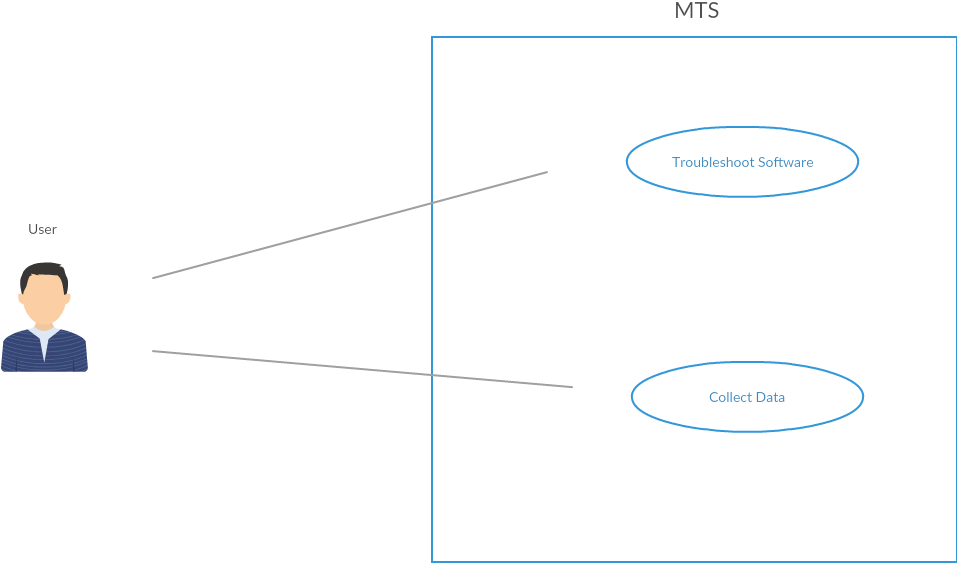
\includegraphics[scale=0.69]{MTS.png}
\end{center}
\newline

\begin{tabular}{|p{5 cm}|p{5 cm}|p{5 cm}|}
	\hline
	\textbf{Requirement ID}: \newline Troubleshoot software & \textbf{Requirement Type}: \newline Functional & \textbf{Scenario ID(s)}: \newline TS 
	\\\hline
	\multicolumn{3}{|p{15cm}|}{\textbf{Requirement}: The software designed shall have the capability of troubleshooting issues with the MTS.}
	\\\hline
	\multicolumn{3}{|p{15cm}|}{\textbf{Rationale}: When the MTS isn’t functioning correctly, the software must be able to provide a reason to the user.}
	\\\hline
	\multicolumn{3}{|p{15cm}|}{\textbf{Source}: Client}
	\\\hline
	\multicolumn{3}{|p{15cm}|}{\textbf{Acceptance Criterion}: When the MTS isn’t functioning, the script provides a reason in all test cases.}
	\\\hline
	\multicolumn{2}{|p{10cm}|}{\textbf{Dependencies}: MTS is not functioning} &
	\textbf{Conflicts}: N/A
	\\\hline
	\multicolumn{3}{|p{15cm}|}{\textbf{Supporting Materials}: Requirements Document, Client}
	\\\hline
	\multicolumn{3}{|p{15cm}|}{\textbf{Modification History}: Last Modified 9/30/18}
	\\\hline
\end{tabular}

\begin{tabular}{|p{5 cm}|p{5 cm}|p{5 cm}|}
	\hline
	\textbf{Requirement ID}: \newline Configure Software & \textbf{Requirement Type}: \newline Functional & \textbf{Scenario ID(s)}: \newline CS 
	\\\hline
	\multicolumn{3}{|p{15cm}|}{\textbf{Requirement}: The software designed shall configure the MTS based on the user’s required functionality.}
	\\\hline
	\multicolumn{3}{|p{15cm}|}{\textbf{Rationale}:The user must be able to easily start the MTS and collect data. Without a configuration script, the user would have to manually move data from one application to another.}
	\\\hline
	\multicolumn{3}{|p{15cm}|}{\textbf{Source}: Client}
	\\\hline
	\multicolumn{3}{|p{15cm}|}{\textbf{Acceptance Criterion}: Data is moved autonomously between software applications DATE, ROOT, and AMORE.}
	\\\hline
	\multicolumn{2}{|p{10cm}|}{\textbf{Dependencies}: N/A} &
	\textbf{Conflicts}: N/A
	\\\hline
	\multicolumn{3}{|p{15cm}|}{\textbf{Supporting Materials}: Requirements Document, Client}
	\\\hline
	\multicolumn{3}{|p{15cm}|}{\textbf{Modification History}: Last Modified 9/30/18}
	\\\hline
\end{tabular}

\newpage
\subsection*{MTS Class Diagram:} 
\addcontentsline{toc}{subsection}{\protect\numberline{}MTS Class Diagram}%
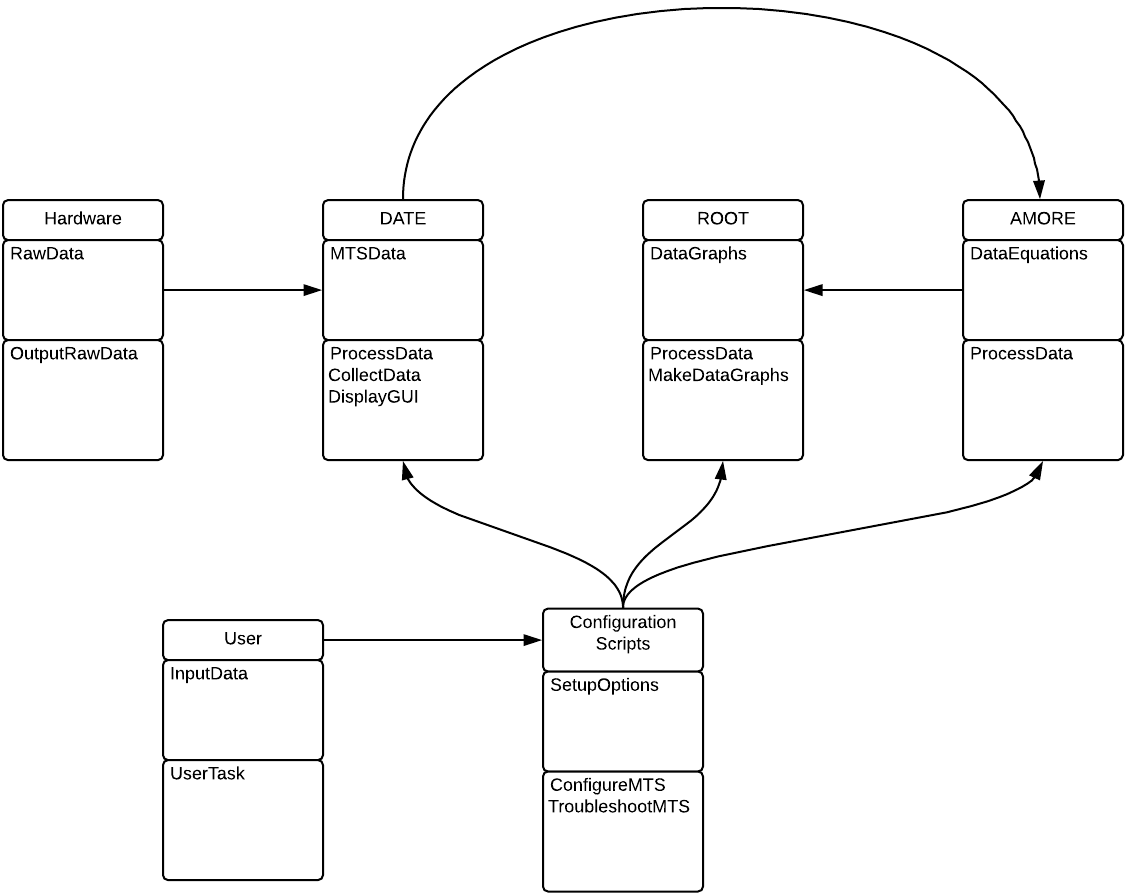
\includegraphics[scale=.90]{MTSCLASS.png}
\newline \\
\subsection*{UML}
\addcontentsline{toc}{subsection}{\protect\numberline{}UML}%
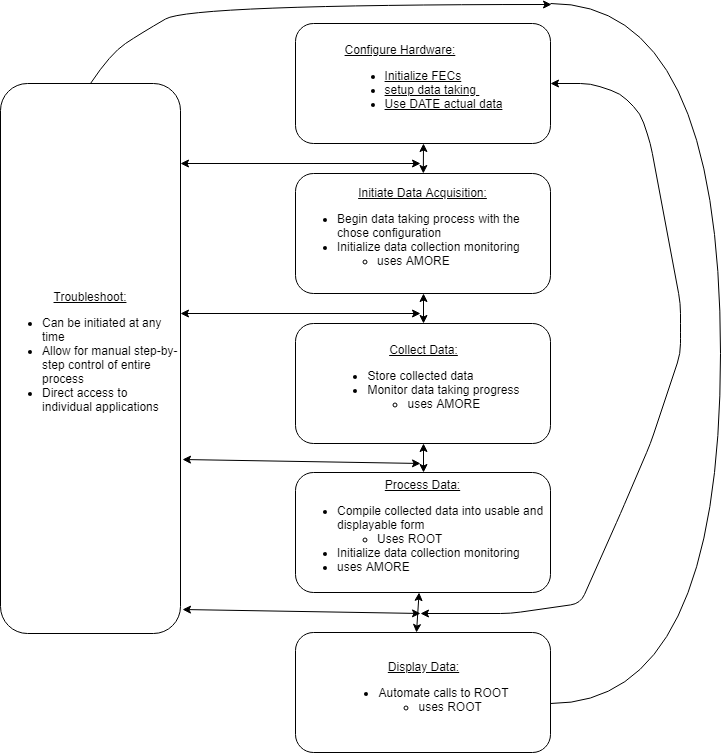
\includegraphics[scale=.6]{DIAGRAM.png}


\section*{Cluster}
\addcontentsline{toc}{section}{\protect\numberline{}Cluster}%

\subsection*{Software Overview:}
\addcontentsline{toc}{subsection}{\protect\numberline{}Software Overview}%
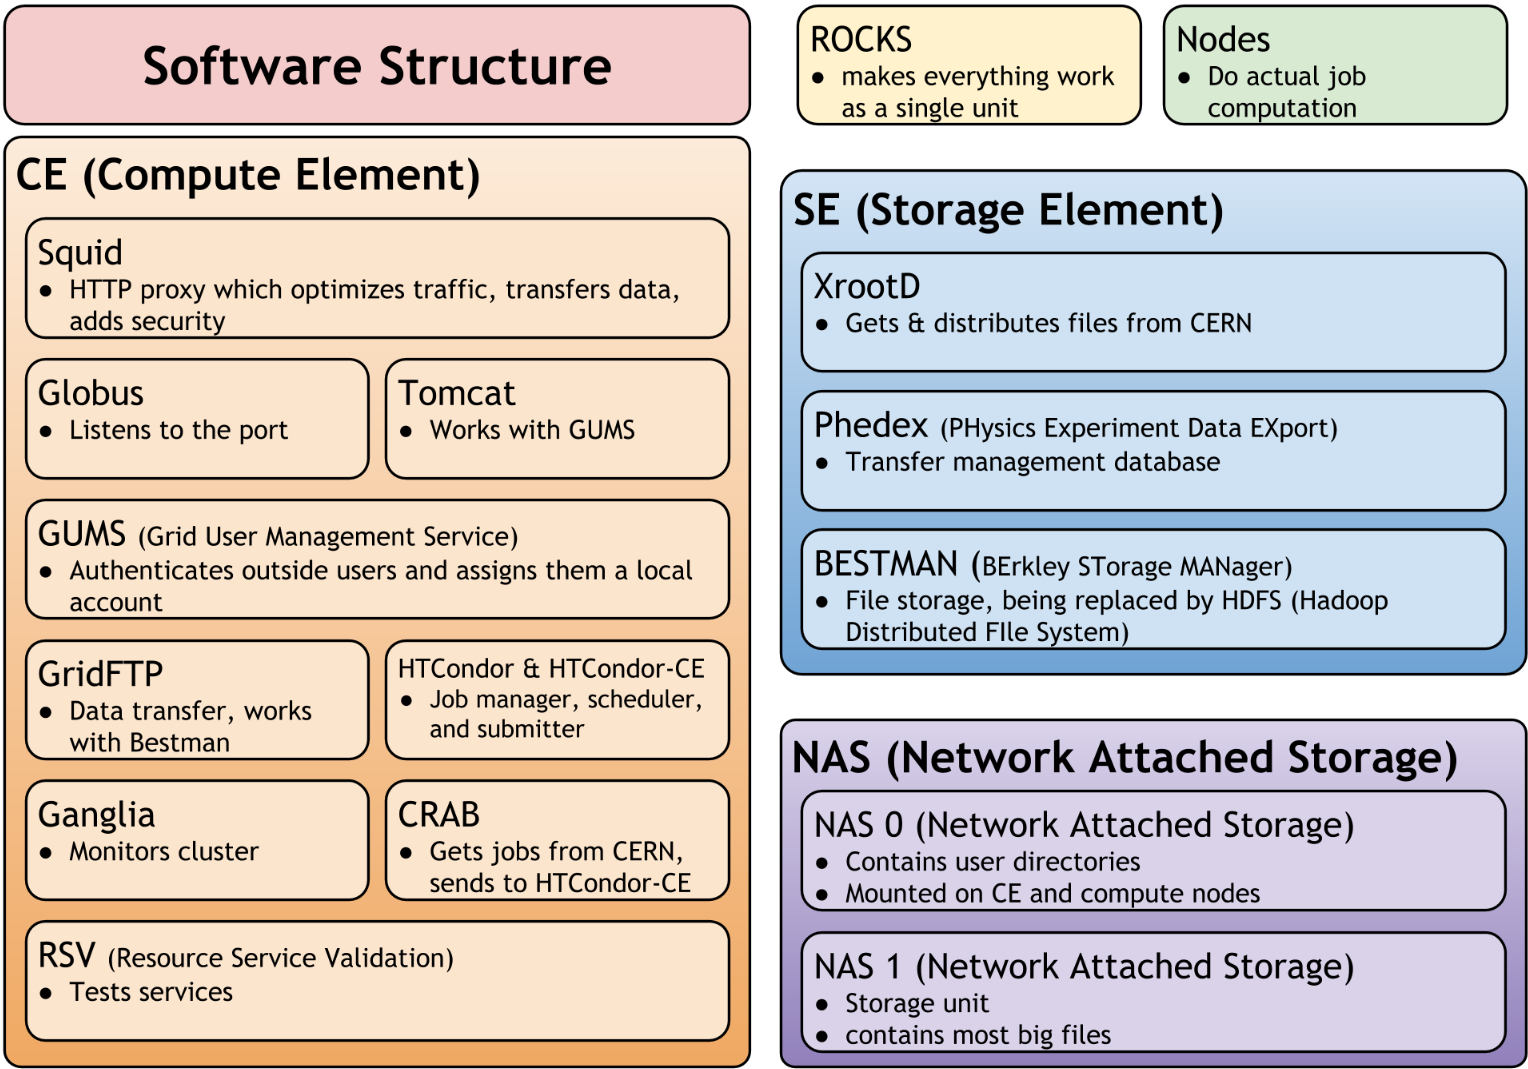
\includegraphics[scale=.4]{ClusterStructure.png}
\newline
\subsection*{Cluster Use Case Diagram:}
\addcontentsline{toc}{subsection}{\protect\numberline{}Cluster Use Case Diagram}%
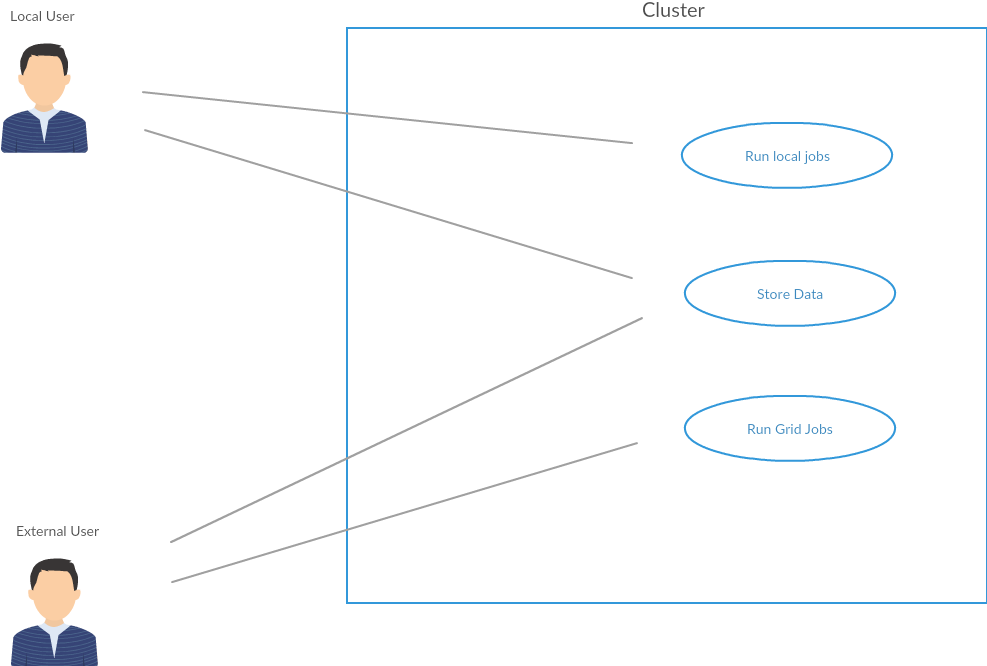
\includegraphics[scale=.67]{Cluster.png}
%\section*{GEM Machines}
%\addcontentsline{toc}{section}{\protect\numberline{}GEM Machines}%

%\subsection*{Allocation Of Resources}
%\addcontentsline{toc}{subsection}{\protect\numberline{}Allocation Of Resources}%

\end{document}
